% =====================================================================
%  Capítulo 5 — Conectividade e conjunto de dados (existe a partir da AP2)
%  Versão 2026.2-AP2 (17/10/2026)
% =====================================================================
\chapter{Conectividade e conjunto de dados}
\label{cap:conectividade}
\rubricaJustificativa

\begin{orientacao}
Este capítulo só é compilado com \texttt{\textbackslash def\textbackslash CICLO\{2\}}
(ou \texttt{\{3\}}) em \texttt{config/dados-da-equipe.tex}. Ele documenta
o \moduloDoCiclo: como o sistema da AP1 passou a falar com o mundo e o
que ele coletou na campanha de 19 a 25/10.

\textbf{Quase nada aqui é escrito do zero.} Cada seção corresponde a um
instrumento que a equipe já entregou no módulo: a matriz de decisão
(22/09), o contrato de dados (23/09), o contrato de tópicos (29/09), o
checklist de prontidão (06/10), o contrato GATT (09/10) e a folha da
conta do ar (07/10). O trabalho é \textbf{transcrever a versão
atualizada}, corrigida pelo que a equipe aprendeu depois, e não colar a
versão entregue. Uma decisão que mudou é informação; diga quando e por
quê ela mudou.
\end{orientacao}

% ---------------------------------------------------------------------
\section{Tecnologia de comunicação}
\label{sec:tecnologia}
\rubricaJustificativa

\begin{orientacao}
A matriz de 22/09, atualizada. Use as três marcas da aula (\serve,
\ressalva, \naoserve) e não some pontos: os cinco critérios não se
convertem uns nos outros. A coluna \enquote{O que o projeto exige} leva
\textbf{um número do seu projeto} (metros, mA$\cdot$h/dia, bytes por
mensagem, segundos), e não uma qualidade.

Duas linhas costumam ter mudado depois de 22/09: a do \textbf{BLE},
depois do contrato GATT e da demo em casa (05/10), e a do
\textbf{LoRa/LoRaWAN}, depois da conta do ar (07/10). A
Tabela~\ref{tab:mudancas} registra essas mudanças.
\end{orientacao}

A matriz de 22/09 apontava LoRa/LoRaWAN, pela energia e pela penetração
na parede do freezer, e a escolha se manteve. O módulo LoRa comprado pela
equipe não chegou a tempo para este ciclo. No lugar dele, a equipe
testou em 24/10 os dois rádios do próprio ESP32, ESP-NOW e BLE, nas
mesmas distâncias e obstáculos. O ESP-NOW foi bem até \SI{8}{\metre} com
uma parede, mas os dois perderam pacotes a partir de duas paredes, e
nenhum foi testado através da parede metálica de um freezer, o caso que
o produto precisa cobrir. A Tabela~\ref{tab:matriz} é a matriz atualizada, com um
número do projeto em cada exigência; a Tabela~\ref{tab:mudancas}
registra as marcas revistas depois dos testes, e por quê; e a decisão,
com a condição em que ela deixaria de valer, vem logo depois, na
\DP{8}. Em uma frase: LoRa entre os nós de borda e o nó central do
produto, quando o módulo chegar; WiFi com MQTT para o nó desta campanha,
na tomada e perto do roteador, porque era o rádio disponível.

{\scriptsize \setlength{\tabcolsep}{3pt}
\begin{longtable}{@{}L{2.3cm}L{2.9cm}C{1.45cm}C{1.45cm}C{1.55cm}C{1.55cm}L{2.6cm}@{}}
\caption{Matriz de decisão de conectividade}\label{tab:matriz}\\
\toprule
\textbf{Critério} & \textbf{O que o projeto exige} & \textbf{WiFi} & \textbf{BLE}
& \textbf{LoRa/ LoRaWAN} & \textbf{NB-IoT/ LTE-M} & \textbf{Observação} \\
\midrule
\endfirsthead
\multicolumn{7}{@{}l}{\footnotesize\itshape Tabela~\ref{tab:matriz} --- continuação}\\
\toprule
\textbf{Critério} & \textbf{O que o projeto exige} & \textbf{WiFi} & \textbf{BLE}
& \textbf{LoRa/ LoRaWAN} & \textbf{NB-IoT/ LTE-M} & \textbf{Observação} \\
\midrule
\endhead
\midrule
\multicolumn{7}{@{}r}{\footnotesize\itshape continua na próxima página}\\
\endfoot
\bottomrule
\endlastfoot
Alcance necessário        & na campanha, o roteador no mesmo ambiente do nó (RSSI de \SI{-15}{} a \SI{-29}{dBm}); no produto, do nó de borda ao nó central, com o nó de borda dentro de um freezer ou câmara fria, de paredes metálicas, a uma distância ainda desconhecida (a planta da farmácia não foi levantada, Seção~\ref{sec:local})
  & \ressalva & \naoserve & \serve & \serve
  & rádio de \SI{2,4}{\giga\hertz} do ESP32 (ESP-NOW): 0\,\% de perda até \SI{8}{\metre} com 1 parede, 18,7\,\% a \SI{11}{\metre} com 2 e 97,6\,\% a \SI{18}{\metre}; BLE: 40\,\% a \SI{11}{\metre}, sem enlace a \SI{13}{\metre}; freezer não testado; LoRa: \SI{915}{\mega\hertz}, matriz de 22/09 \\
Energia disponível        & 18650 de \SI{2600}{\mAh} (\SI{2080}{\mAh} úteis); \SI{69,4}{\mAh}/dia já gastos sem rádio (Apêndice~\ref{ap:energia})
  & \ressalva & \serve & \serve & \naoserve
  & WiFi: +\SI{29,7}{\mAh}/dia medidos e 30 $\rightarrow$ 21 dias; ESP-NOW: $\approx$\SI{0,14}{\mAh}/dia; BLE ($\approx$\SI{1}{\mAh}/dia), LoRa ($\approx$2--3) e NB-IoT ($\approx$25--30): folha de dados, matriz de 22/09 \\
Dado por transmissão      & 73 bytes de JSON (ou 8 em binário) a cada \SI{600}{\second} (\RF{01}): 144 mensagens/dia
  & \serve & \serve & \ressalva & \serve
  & LoRa: o JSON não cabe de SF10 a SF12 (máx. 51 bytes); 8 bytes cabem até SF9 \\
Latência aceitável        & o alarme é local (\DP{5}); a leitura precisa chegar ao gravador antes da seguinte (\SI{600}{\second})
  & \serve & \serve & \serve & \serve
  & pior medido: 4 a \SI{6}{\second} (BLE congestionado a \SI{11}{\metre}) \\
Infraestrutura no local   & WiFi 2,4 GHz do estabelecimento, de terceiros (exige credenciais e permissão); hardware comprado pela equipe: ESP32 e um módulo LoRa encomendado, que não chegou a tempo; nenhum modem celular
  & \serve & \ressalva & \ressalva & \naoserve
  & BLE precisa de um central por ambiente; LoRa precisa do módulo em cada nó e de um nó central com rádio LoRa; NB-IoT, de modem e plano de dados \\
Custo do rádio por ponto  & $\leq$ R\$\,44,80 (o teto de R\$\,150,00 do \RNF{03} menos os R\$\,105,20 já gastos)
  & \serve & \serve & \ressalva & \naoserve
  & WiFi e BLE já vêm no ESP32; módulo LoRa de R\$\,40 a 60, mais o \emph{gateway}; NB-IoT: módulo de R\$\,90 ou mais e plano de dados \\
Interferência (\RNF{05}) & conviver com compressor e ar-condicionado junto ao nó
  & \ressalva & \ressalva & \serve & \serve
  & \SI{2,4}{\giga\hertz} é a faixa mais congestionada; na campanha, \SI{33}{\minute} de ar ligado sem salto entre leituras e com RSSI forte \\
\end{longtable}
\vspace{-0.6\baselineskip}
\fonte{Elaborada pela equipe: a matriz de 22/09/2026 (\texttt{docs/anexos/matriz-decisao-22-09-2026.pdf}), com os sete critérios de então, atualizada com as medições do Módulo~2.}
}

{\footnotesize \setlength{\tabcolsep}{3.5pt}
\begin{longtable}{@{}L{3.0cm}L{1.7cm}L{1.7cm}L{7.6cm}@{}}
\caption{Marcas revistas depois de 22/09}\label{tab:mudancas}\\
\toprule
\textbf{Tecnologia · critério} & \textbf{Em 22/09} & \textbf{Agora} & \textbf{O que mudou ou confirmou a marca} \\
\midrule
\endfirsthead
\multicolumn{4}{@{}l}{\footnotesize\itshape Tabela~\ref{tab:mudancas} --- continuação}\\
\toprule
\textbf{Tecnologia · critério} & \textbf{Em 22/09} & \textbf{Agora} & \textbf{O que mudou ou confirmou a marca} \\
\midrule
\endhead
\midrule
\multicolumn{4}{@{}r}{\footnotesize\itshape continua na próxima página}\\
\endfoot
\bottomrule
\endlastfoot
WiFi · alcance & \ressalva & \ressalva & Mantida. Na campanha, com o roteador no mesmo cômodo, o RSSI ficou entre \SI{-15}{} e \SI{-29}{dBm}. Mas o mesmo rádio, em ESP-NOW, perdeu 18,7\,\% dos pacotes a \SI{11}{\metre} com duas paredes e 97,6\,\% a \SI{18}{\metre} (bateria de 24/10), e o interior do freezer, o ponto mais difícil do cenário, continua não testado. \\
WiFi · energia & \naoserve & \ressalva & A estimativa de 22/09 (20 a \SI{30}{\mAh}/dia) foi confirmada pela medição: \SI{29,7}{\mAh}/dia no pior ciclo, autonomia de 21 dias. Não serve para o nó a bateria sozinho, mas serve no nó na tomada (a campanha) e no nó central do produto. \\
WiFi · infraestrutura & \naoserve{} sem AP & \serve & Há WiFi 2,4\,GHz no estabelecimento e no local da campanha; a ressalva das credenciais fica nas restrições (Seção~\ref{cap:requisitos}). \\
BLE · alcance & \naoserve & \naoserve & Mantida, agora com medição. Bateria de 24/10, nas mesmas posições do ESP-NOW, a +\SI{9}{dBm} (o máximo do BLE no ESP32): 100\,\% entregue até \SI{8}{\metre}, com latência de \SI{16}{\milli\second} contra \SI{1,9}{\milli\second}; a \SI{11}{\metre}, só 40\,\%, com 4 a \SI{6}{\second} de atraso, porque a fila do BLE congestiona; sem enlace a \SI{13}{\metre}. Chegou cerca de \SI{8,7}{\deci\bel} mais fraco que o ESP-NOW. O pacote de 25 bytes exigiu MTU de 64; o central foi um segundo ESP32. \\
LoRa · dado por transmissão & \serve & \ressalva & Em 22/09, o bloco era de $\approx$12 bytes. Pela conta do ar da Aula~14 (AU915, \SI{125}{\kilo\hertz}, uso justo de \SI{30}{\second}/dia na TTN), 8 bytes de aplicação (+13 de cabeçalho) levam \SI{57}{\milli\second} em SF7 ($\approx$530 mensagens/dia) e \SI{1,48}{\second} em SF12 ($\approx$20/dia): os 144/dia cabem até SF9 ($\approx$160/dia). O JSON de 73 bytes da campanha não cabe de SF10 a SF12 (máximo de 51 bytes). \\
LoRa · infraestrutura & \ressalva & \ressalva & Mantida. A equipe comprou um módulo LoRa, que não chegou a tempo para este ciclo; o produto precisa ainda de um nó central com rádio LoRa (ou de um \emph{gateway} LoRaWAN próprio, ligado à internet; a cobertura da TTN em Teresina não foi verificada). \\
NB-IoT · infraestrutura & \ressalva & \naoserve & A equipe não tem modem celular, e o módulo com plano de dados estoura o custo por ponto. \\
Zigbee & não avaliado & \naoserve & Citado na AP1 como alternativa. O ESP32 usado no protótipo integra só WiFi e Bluetooth \cite{rahman2026esp32review}, sem rádio IEEE~802.15.4 (só o ESP32-C6 e o H2 têm): exigiria um módulo à parte e um coordenador ligado à internet, o mesmo degrau do nó central, sem usar o rádio que já está na placa. \\
\end{longtable}
\vspace{-0.6\baselineskip}
\fonte{Elaborada pela equipe, a partir da matriz de 22/09/2026
  (\texttt{docs/anexos/matriz-decisao-22-09-2026.pdf}). As marcas que não
  aparecem aqui não foram revistas.}
}

\begin{orientacao}
Agora a decisão, numa caixa \DP{n}. Uma justificativa aceitável diz
\textbf{em que condição a escolha deixaria de valer}; \enquote{escolhemos
WiFi porque o ESP32 já tem WiFi} não diz. Descartar com motivo vale
tanto quanto escolher: um descarte bem feito, com número, é evidência de
domínio do conteúdo.

O kit da disciplina não tem módulo LoRa. Se a matriz aponta LoRaWAN como
a tecnologia certa para o projeto, essa é uma conclusão legítima: diga
isso, faça a campanha com WiFi e MQTT e declare a diferença como
limitação no Capítulo~\ref{cap:conclusao}. O caminho do dado depois do
servidor de rede (TTN $\rightarrow$ HiveMQ $\rightarrow$ gravador) é o
mesmo da Aula~14.
\end{orientacao}

\begin{decisao}{Tecnologia de comunicação}
\alternativas{WiFi, BLE, ESP-NOW (o rádio WiFi do ESP32 sem roteador nem
  associação, ponto a ponto \cite{zbotic2025espnow}), LoRa/LoRaWAN e
  NB-IoT/LTE-M.}
\criterio{Distância e obstáculos entre o nó de borda e o primeiro ponto
  com internet, inclusive no ponto mais difícil do cenário, dentro de um
  freezer ou câmara fria; orçamento de energia do
  Apêndice~\ref{ap:energia}; bytes e frequência das mensagens;
  infraestrutura existente no local.}
\escolha{Para o produto, \textbf{LoRa} entre os nós de borda e o nó
  central, e WiFi só no nó central, como previa a arquitetura original.
  O módulo LoRa comprado pela equipe não chegou a tempo para este ciclo;
  por isso, a campanha usou o rádio disponível: WiFi, com MQTT sobre TLS
  até o \emph{broker}, com o nó alimentado pela USB e a poucos metros do
  roteador (RSSI mediano de \SI{-18}{dBm}).}
\evidencia{Em 22/09, a matriz apontava LoRa, pela energia (2 a
  \SI{3}{\mAh}/dia, \folhadedados) e pela penetração no freezer
  (\SI{915}{\mega\hertz}). Sem o módulo, a equipe testou em 24/10 os dois
  rádios do ESP32 como substitutos, nas mesmas posições (10 pacotes de 25
  bytes por segundo, \SI{60}{\second} por posição). O ESP-NOW não perdeu
  nenhum de \num{3010} pacotes até \SI{8}{\metre} com uma parede (RSSI
  p10 de \SI{-86}{dBm}, latência mediana de \SI{1,9}{\milli\second}), mas
  perdeu 18,7\,\% a \SI{11}{\metre} com duas paredes e 97,6\,\% a
  \SI{18}{\metre}. O BLE chegou cerca de \SI{8,7}{\deci\bel} mais fraco,
  entregou só 40\,\% a \SI{11}{\metre}, com 4 a \SI{6}{\second} de atraso,
  e não fez enlace a \SI{13}{\metre}. O ESP-NOW serviu bem de perto, mas
  esse resultado pode não se repetir no cenário de referência, que tem
  nós dentro de freezer e câmara fria, de paredes metálicas, a uma
  distância que ainda não se conhece; o interior do freezer não chegou a
  ser testado com nenhum rádio, e o LoRa, em \SI{915}{\mega\hertz},
  atravessa melhor esse tipo de obstáculo (matriz de 22/09). O WiFi direto ao roteador usa o mesmo
  rádio de \SI{2,4}{\giga\hertz} e ainda custa \SI{2,27}{\second} de rádio
  por ciclo na mediana e \SI{2,48}{\second} no pior caso
  (Seção~\ref{sec:custo-radio}): \SI{29,7}{\mAh}/dia e autonomia de 21
  dias. Na campanha de 24/10, com o roteador no mesmo cômodo, o WiFi não
  foi o gargalo: as perdas vieram da conexão com o \emph{broker}, que
  caía em segundos na fase degradada (Seção~\ref{sec:qualidade}).}
\consequencia{O produto depende do módulo LoRa e de um nó central com
  rádio LoRa, que ainda não existem em hardware: o enlace LoRa e o seu
  consumo serão medidos quando o módulo chegar, e até lá a linha do rádio
  do nó de borda é estimativa de folha de dados ($\approx$29 dias de
  autonomia, Apêndice~\ref{ap:energia}), e o custo por ponto sobe para
  R\$\,145,20 a 165,20, no limite do \RNF{03} (Seção~\ref{sec:bom}). O
  contrato tem de virar binário:
  o JSON de 73 bytes não cabe de SF10 a SF12, e 8 bytes cabem até SF9
  (Tabela~\ref{tab:mudancas}). A escolha deixaria de valer se todos os
  nós de um estabelecimento ficassem na mesma sala do nó central, a no
  máximo \SI{8}{\metre} e uma parede: aí o ESP-NOW serviria, com 0\,\% de
  perda medida e com o rádio que o ESP32 já tem. O WiFi da campanha só se
  sustenta com o nó na tomada e perto do roteador.}
\end{decisao}

\begin{exemploguia}
\enquote{O nó fica a \SI{12}{\metre} do roteador do laboratório, na
tomada, e publica \SI{110}{} bytes a cada \SI{30}{\second}. Alcance e
energia não restringem; WiFi serve sem infraestrutura nova. Deixaria de
servir se o nó fosse para o pasto: a \SI{300}{\metre} da sede, WiFi e BLE
caem, e a conta do ar mostra que a leitura agregada de hora em hora
cabe em LoRaWAN até SF10.}
\end{exemploguia}

% ---------------------------------------------------------------------
\section{Caminho do dado, do sensor ao arquivo}
\label{sec:caminho}
\rubricaFuncionalidade

\begin{orientacao}
Um diagrama, do sensor ao CSV, com cada peça no lugar em que ela
\emph{de fato} rodou durante a campanha: o nó, o roteador, o
\emph{broker}, o gravador, o arquivo, o \texttt{qualidade.py}. Ao lado
de cada seta, o protocolo (I\textsuperscript{2}C, WiFi, MQTT sobre TLS na
porta 8883). Depois do diagrama, a tabela diz quem mantém cada peça
ligada e o que se perde quando ela para. É essa tabela que mostra se a
equipe entendeu a frase do Lab~03: \emph{o broker transporta; quem
guarda é quem assina}.
\end{orientacao}

A Figura~\ref{fig:caminho} mostra o caminho que cada leitura percorreu na
campanha, com cada peça no lugar em que de fato rodou e o protocolo de
cada trecho. O nó publica por WiFi e MQTT sobre TLS; o \emph{broker}
público só transporta; quem guarda é o gravador, que assina com sessão
persistente e escreve uma linha por mensagem no CSV. A
Tabela~\ref{tab:pecas} diz quem mantém cada peça ligada e o que se perde
quando ela para. O caminho do produto tem dois trechos a mais: o LoRa
até o nó central, que espera o módulo (os substitutos testados estão na
Seção~\ref{sec:espnow-bancada}), e o envio em lote até o servidor, já
exercitado com as leituras da campanha (Seção~\ref{sec:ponte}).

\begin{figure}[H]
\centering
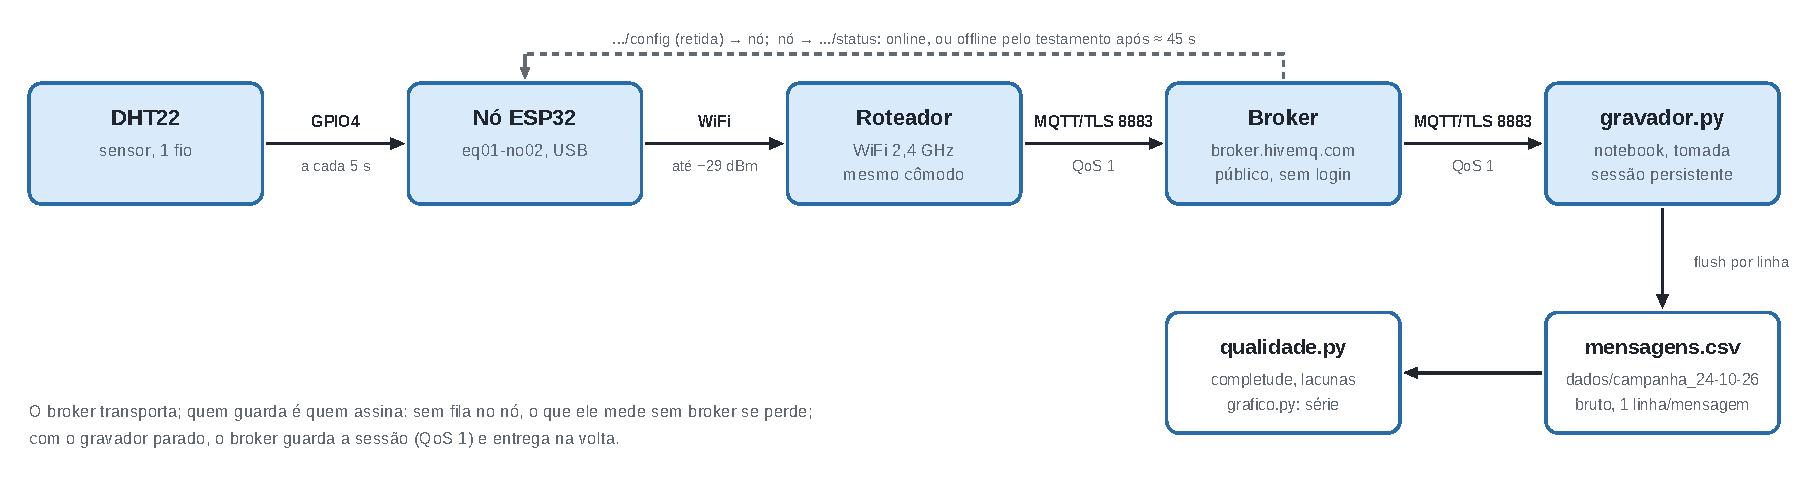
\includegraphics[width=\textwidth]{figuras/caminho-do-dado.pdf}
\caption{Caminho do dado durante a campanha de coleta}
\label{fig:caminho}
\fonte{Elaborada pela equipe.}
\end{figure}

{\footnotesize
\begin{longtable}{@{}L{2.4cm}L{3.4cm}L{3.0cm}L{5.2cm}@{}}
\caption{Onde roda cada peça, e o que acontece se ela parar}\label{tab:pecas}\\
\toprule
\textbf{Peça} & \textbf{Onde rodou} & \textbf{Alimentação} & \textbf{Se parar, o que se perde} \\
\midrule
\endfirsthead
\multicolumn{4}{@{}l}{\footnotesize\itshape Tabela~\ref{tab:pecas} --- continuação}\\
\toprule
\textbf{Peça} & \textbf{Onde rodou} & \textbf{Alimentação} & \textbf{Se parar, o que se perde} \\
\midrule
\endhead
\midrule
\multicolumn{4}{@{}r}{\footnotesize\itshape continua na próxima página}\\
\endfoot
\bottomrule
\endlastfoot
Nó ESP32       & escrivaninha, no mesmo cômodo do ar-condicionado e fora do fluxo de ar dele, na residência de João Pedro Saleh & USB & O que o nó mede enquanto está desligado nunca existe. O \texttt{status} vira \texttt{offline} em cerca de \SI{45}{\second} (\SI{46}{\second} no \CT{10}). O \emph{firmware} da campanha não tem alarme local. \\
Roteador       & o mesmo ambiente (RSSI de \SI{-15}{} a \SI{-29}{dBm}) & rede elétrica do local & O nó não alcança o \emph{broker} e, sem fila local, não mede: na queda de \SI{101}{\second} do \CT{09}, cerca de 19 leituras deixaram de existir. \\
\emph{Broker}  & público, \texttt{broker.hivemq.com}, sem autenticação & --- & Nó e gravador perdem o único elo entre eles; nada do período é guardado em lugar nenhum. \\
Gravador       & notebook de João Pedro Saleh, no mesmo local & tomada (notebook carregando) & Nada, por um tempo: com sessão persistente, \emph{client ID} fixo e QoS~1, o \emph{broker} guarda as mensagens e as entrega na volta. Na campanha, o gravador começou \SI{8,7}{\minute} depois do nó, e as 100 leituras desse intervalo chegaram juntas, com o \texttt{ts} original (\CT{12}). O \emph{broker} público não publica por quanto tempo guarda uma sessão. \\
\end{longtable}
\vspace{-0.6\baselineskip}
\fonte{Elaborada pela equipe.}
}

% ---------------------------------------------------------------------
\section{Contrato de dados}
\label{sec:contrato-dados}
\rubricaJustificativa

\begin{orientacao}
O JSON que o nó publica, na versão que rodou na campanha. Uma linha por
chave. As quatro primeiras são as da disciplina e já vêm preenchidas:
confira se o seu nó as publica exatamente assim. As demais são as
grandezas do projeto, \textbf{com a unidade no nome da chave}
(\texttt{temp\_c}, \texttt{umid\_pct}, \texttt{acel\_g}). Se o contrato
mudou durante o módulo, diga qual é a versão e o que mudou.
\end{orientacao}

{\footnotesize \setlength{\tabcolsep}{3.5pt}
\begin{longtable}{@{}L{2.3cm}L{1.8cm}L{2.2cm}L{2.4cm}L{5.4cm}@{}}
\caption{Contrato de dados da telemetria (versão 2, a da campanha)}\label{tab:contrato-dados}\\
\toprule
\textbf{Chave} & \textbf{Tipo} & \textbf{Unidade} & \textbf{Exemplo} & \textbf{Para que serve} \\
\midrule
\endfirsthead
\multicolumn{5}{@{}l}{\footnotesize\itshape Tabela~\ref{tab:contrato-dados} --- continuação}\\
\toprule
\textbf{Chave} & \textbf{Tipo} & \textbf{Unidade} & \textbf{Exemplo} & \textbf{Para que serve} \\
\midrule
\endhead
\midrule
\multicolumn{5}{@{}r}{\footnotesize\itshape continua na próxima página}\\
\endfoot
\bottomrule
\endlastfoot
\texttt{id}   & texto   & ---    & \texttt{eq01-no02} & identifica o nó (\texttt{<equipe>-<nó>}, o mesmo do tópico); parte da chave de deduplicação \\
\texttt{boot} & inteiro & ---    & ---                & \textbf{ausente na versão da campanha.} Mudaria a cada ligamento e separaria um reinício de uma perda; entra na versão~3 (\CT{11}) \\
\texttt{seq}  & inteiro & ---    & \texttt{100}       & conta as leituras e recomeça em 1 a cada ligamento; o salto denuncia a publicação que falhou, a repetição denuncia a duplicata \\
\texttt{ts}   & inteiro & s (época Unix) & \texttt{1792869010} & instante da leitura no nó (NTP), em UTC; \texttt{null} antes de sincronizar \\
\texttt{temp\_c}   & real & \si{\celsius} & \texttt{25.3} & temperatura do DHT22, leitura única por período, uma casa decimal (a resolução do sensor); ausente se a leitura falhou \\
\texttt{umid\_pct} & real & \% UR & \texttt{35.7} & umidade relativa do DHT22, uma casa decimal; ausente se a leitura falhou \\
\texttt{rssi\_dbm} & inteiro & dBm & \texttt{-17} & só quando a leitura do DHT22 falha, no lugar das duas grandezas: a mensagem continua marcando o \texttt{seq} e informa a força do sinal no ponto do nó \\
\end{longtable}
\vspace{-0.6\baselineskip}
\fonte{Elaborada pela equipe, a partir do contrato de 23/09/2026 e do
  \emph{firmware} da campanha (\texttt{wokwi/sketch/sketch.ino}, branch
  \texttt{lab3}, \emph{commit} \texttt{7b4482e}).}
}

O contrato mudou uma vez neste módulo. A versão~1, de 23/09 (Aula~10),
foi exercitada em HTTP contra um servidor de eco em 23/10: uma mensagem
dessa versão tem 73 bytes (Listagem~\ref{lst:payload}) e, enviada por
POST, voltou do servidor idêntica campo a campo. A versão~2, a que
rodou na campanha (Listagem~\ref{lst:payload2}), troca o \texttt{id}
fixo (\texttt{termo-no01}) pelo padrão \texttt{<equipe>-<nó>} do Lab~03
e, quando o DHT22 falha, publica \texttt{rssi\_dbm} no lugar das
grandezas, em vez de \texttt{null}. Foram 50 dessas mensagens nas
\num{1263} da campanha (4,0\,\%).

A versão~2 \textbf{não tem o \texttt{boot}}. Sem ele, um reinício zera o
\texttt{seq}, e uma chave de deduplicação (\texttt{id}, \texttt{seq})
descartaria leituras válidas como se fossem repetidas: aplicada aos
arquivos de 24/10, ela teria jogado fora 1 leitura da campanha e 8 dos
testes de falha, nos três reinícios. O \texttt{qualidade.py} contorna
isso separando o arquivo em trechos quando o \texttt{seq} volta a 1 ou 2
(Seção~\ref{sec:qualidade}), o que só funciona se a primeira leitura
depois do reinício chegar. A versão~3 acrescenta o \texttt{boot}, e a
chave passa a ser (\texttt{id}, \texttt{boot}, \texttt{seq}).

\begin{lstlisting}[style=terminal,
  caption={Uma mensagem real da versão 1 do contrato (sessão de 23/10, branch \texttt{apendice\_b})},
  label={lst:payload}]
{"id":"termo-no01","seq":8,"ts":1792787350,"temp_c":25.4,"umid_pct":35.5}
\end{lstlisting}

\begin{lstlisting}[style=terminal,
  caption={Duas mensagens reais da versão 2, copiadas do CSV da campanha: uma leitura normal e uma com o DHT22 em falha},
  label={lst:payload2}]
{"id":"eq01-no02","seq":100,"ts":1792869010,"temp_c":25.3,"umid_pct":35.7}
{"id":"eq01-no02","seq":7,"ts":1792868539,"rssi_dbm":-17}
\end{lstlisting}

\begin{orientacao}
Se o projeto usa (ou avaliou) BLE, transcreva também o contrato GATT de
09/10: serviço, características, formato e ordem dos bytes, escala. Se
não usa, uma frase basta: \enquote{BLE foi descartado (Tabela~\ref{tab:mudancas});
o contrato GATT está na pasta \texttt{aula13} do repositório}.
\end{orientacao}

O BLE foi avaliado e descartado (Tabela~\ref{tab:mudancas}). O contrato
GATT usado na bateria de 24/10 (branch \texttt{teste-ble}, arquivo
\texttt{firmware/comum/pacote.h}) é o da Tabela~\ref{tab:gatt}: o sensor
é o periférico e anuncia o nome \texttt{TermoStats-sensor}; o
\emph{gateway} é o central, conecta, negocia MTU de 64 (o padrão de 23
só carrega 20 bytes por notificação) e assina as notificações. O
mesmo pacote foi usado no teste de ESP-NOW, para que os dois rádios
fossem comparados com a mesma carga. O contrato GATT do exercício de
09/10 não foi arquivado no repositório; o da Tabela~\ref{tab:gatt} é o
que foi de fato exercitado em hardware, e é o que vale para este
relatório.

\begin{table}[H]
\centering
\caption{Contrato GATT da bateria de BLE (24/10)}
\label{tab:gatt}
\footnotesize
\setlength{\tabcolsep}{3.5pt}
\begin{tabular}{@{}L{3.2cm}L{2.4cm}L{2.0cm}L{6.4cm}@{}}
\toprule
\textbf{Item} & \textbf{Tipo} & \textbf{Bytes} & \textbf{Formato e escala} \\
\midrule
Serviço & UUID & --- & \texttt{6e1a0001-7d3f-4b6a-9c4e-2f1b8a5d0c01} \\
Dados (sensor $\rightarrow$ \emph{gateway}) & \emph{notify} & 25 & \texttt{6e1a0002-7d3f-4b6a-9c4e-2f1b8a5d0c01}; estrutura empacotada, \emph{little-endian} \\
ACK (\emph{gateway} $\rightarrow$ sensor) & \emph{write} sem resposta & 9 & \texttt{6e1a0003-7d3f-4b6a-9c4e-2f1b8a5d0c01}; \texttt{tipo}, \texttt{seq} confirmado e \texttt{t\_envio\_us} ecoado \\
\midrule
\texttt{tipo} & \texttt{uint8} & 1 & 1 = dado, 2 = ACK \\
\texttt{seq} & \texttt{uint32} & 4 & avança a cada \SI{100}{\milli\second}, conectado ou não: o buraco é a perda \\
\texttt{t\_envio\_us} & \texttt{uint32} & 4 & \texttt{micros()} do sensor no envio \\
\texttt{rtt\_us}, \texttt{seq\_rtt} & \texttt{uint32} & 4 + 4 & ida e volta medida no último ACK, e a qual \texttt{seq} ela se refere \\
\texttt{tx\_falhas} & \texttt{uint32} & 4 & pacotes não enviados desde o \emph{boot} \\
\texttt{temp\_c\_x10} & \texttt{int16} & 2 & \si{\celsius} $\times$ 10 (\num{26.1} $\rightarrow$ 261); \texttt{INT16\_MIN} = leitura inválida \\
\texttt{umid\_pct\_x10} & \texttt{uint16} & 2 & \% UR $\times$ 10; \texttt{UINT16\_MAX} = leitura inválida \\
\bottomrule
\end{tabular}
\fonte{Elaborada pela equipe, a partir de \texttt{firmware/comum/pacote.h} (branch \texttt{teste-ble}).}
\end{table}

Só os dois últimos campos (4 bytes) são dado do projeto; os outros 21
existem para medir o enlace. Em produção, com \texttt{boot} e
\texttt{seq} de 2 bytes, o pacote cabe em 8 bytes, o tamanho usado na
conta do ar da Tabela~\ref{tab:mudancas}.

% ---------------------------------------------------------------------
\section{Contrato de tópicos e garantias de entrega}
\label{sec:topicos}
\rubricaJustificativa

\begin{orientacao}
O contrato de 29/09, na versão da campanha. A coluna \enquote{Por quê}
é a que o docente lê primeiro: uma frase por linha. Lembretes da Aula 11:
o QoS efetivo de uma entrega é o \textbf{menor} entre o de quem publica e
o de quem assina; QoS~1 pode entregar duas vezes, e é o \texttt{seq} que
permite descartar a duplicata; telemetria retida faz um painel recém-aberto
mostrar uma leitura velha como se fosse atual.
\end{orientacao}

{\scriptsize \setlength{\tabcolsep}{3pt}
\begin{longtable}{@{}L{3.6cm}L{1.9cm}C{0.8cm}C{1.1cm}L{2.4cm}L{4.0cm}@{}}
\caption{Contrato de tópicos MQTT}\label{tab:topicos}\\
\toprule
\textbf{Tópico} & \textbf{Direção} & \textbf{QoS} & \textbf{Retido?} & \textbf{Quem assina} & \textbf{Por quê} \\
\midrule
\endfirsthead
\multicolumn{6}{@{}l}{\footnotesize\itshape Tabela~\ref{tab:topicos} --- continuação}\\
\toprule
\textbf{Tópico} & \textbf{Direção} & \textbf{QoS} & \textbf{Retido?} & \textbf{Quem assina} & \textbf{Por quê} \\
\midrule
\endhead
\midrule
\multicolumn{6}{@{}r}{\footnotesize\itshape continua na próxima página}\\
\endfoot
\bottomrule
\endlastfoot
\texttt{ufpi-iot26/\allowbreak eq01/\allowbreak no02/\allowbreak telemetria} & nó $\rightarrow$ \emph{broker} & 1 & não & gravador & QoS~1 garante a entrega nas duas pernas; a cópia que ele pode gerar sai pela chave (\texttt{id}, \texttt{seq}) dentro de cada trecho entre reinícios, enquanto não houver \texttt{boot}. Retida, faria um painel recém-aberto mostrar uma leitura velha como atual. \\
\texttt{ufpi-iot26/\allowbreak eq01/\allowbreak no02/\allowbreak status}     & nó $\rightarrow$ \emph{broker} (e testamento) & 1 & sim & gravador; MQTT Explorer, para ver ao vivo & Retido, quem chega depois vê o estado atual na hora; o testamento publica \texttt{offline} quando o nó cai sem avisar. \\
\texttt{ufpi-iot26/\allowbreak eq01/\allowbreak no02/\allowbreak config}     & \emph{broker} $\rightarrow$ nó & 1 & sim & o nó & \texttt{\{\textquotedbl periodo\_s\textquotedbl:N\}}. Retida, o nó que reinicia recebe a configuração logo ao conectar, sem perguntar; mensagem vazia retida volta ao padrão (\SI{5}{\second}). Não foi usada na campanha. \\
\end{longtable}
\vspace{-0.6\baselineskip}
\fonte{Elaborada pela equipe, a partir do contrato de 29/09/2026. Na
  campanha, o nó da placa foi o \texttt{no02}; o \texttt{no01} fica
  reservado para o Wokwi, para que os dois nunca usem o mesmo
  \emph{client ID}.}
}

\begin{orientacao}
Depois da tabela, as quatro decisões que transformam um nó que publica
num nó que forma um conjunto de dados. Cada uma com o número que a
sustenta. Se alguma delas for importante o bastante para o projeto,
promova-a a uma caixa \DP{n}.
\end{orientacao}

\noindent O protocolo da campanha é o MQTT do Lab~03. Comparado a
WebSocket e Firebase no ESP32-C3, sob as mesmas condições, ele teve
desempenho equilibrado e o uso de banda mais eficiente em redes
restritas \cite{yamin2026mqttwsfirebase}; e a sessão persistente, o
QoS e o testamento, que as quatro decisões abaixo usam, são do próprio
protocolo.

\begin{description}[style=unboxed, leftmargin=0pt, font=\normalfont\bfseries]
  \item[1. Sessão persistente ou limpa, no nó e no gravador.]\hfill\\
    Persistente nos dois, com \emph{client ID} fixo:
    \texttt{ufpi-iot26-eq01-no02} no nó e \texttt{ufpi-iot26-eq01-gravador}
    no gravador. É a combinação de sessão persistente, mesmo \emph{client
    ID} e QoS~1 que faz o \emph{broker} guardar as leituras enquanto o
    gravador está parado: na campanha, o gravador foi ligado
    \SI{8,7}{\minute} depois do nó, e as 100 leituras desse intervalo
    chegaram em \SI{3}{\second}, com o \texttt{ts} original. Dois clientes
    com o mesmo ID derrubam um ao outro; por isso a placa e o Wokwi nunca
    usam o mesmo nome de nó.
  \item[2. O que o nó faz com as leituras quando o broker está fora de alcance.]\hfill\\
    Nada: o \emph{firmware} da campanha não tem fila local. Sem
    \emph{broker}, a leitura não é feita, e o \texttt{seq} não avança. Na
    queda de WiFi do \CT{09} (\SI{101}{\second}), cerca de 19 leituras
    deixaram de existir, e o \texttt{seq} pulou só 1; na campanha,
    faltaram cerca de 740 leituras, e o \texttt{seq} acusou 2. A lacuna
    não aparece como salto de \texttt{seq}; só aparece na completude
    (Seção~\ref{sec:qualidade}). Com uma fila de 120 leituras, que em
    binário (\texttt{ts}, \texttt{seq} e as duas grandezas, 12 bytes cada)
    ocupam menos de 1,5\,kB de RAM, o nó cobriria
    \SI{10}{\minute} sem \emph{broker} no período de \SI{5}{\second}, ou 20
    horas no período de \SI{600}{\second} do \RF{01}. Essa fila é a
    principal mudança de \emph{firmware} para o próximo ciclo.
  \item[3. Keepalive e testamento.]\hfill\\
    \emph{Keepalive} de \SI{30}{\second}: um nó que morre sem avisar
    aparece como \texttt{offline} cerca de \SI{45}{\second} depois da
    última mensagem dele (\SI{46}{\second} no \CT{10}). No
    \emph{firmware} da campanha, o laço não tem nenhum \texttt{delay()}
    longo: a leitura do DHT22 é única, e o período é contado com
    \texttt{millis()}. A leitura filtrada da AP1 com o pulso de alarme
    deixaria o laço cerca de \SI{11,4}{\second} sem chamar
    \texttt{mqtt.loop()}, ainda dentro do limite, quando as duas versões
    forem unidas.
  \item[4. Segurança mínima.]\hfill\\
    TLS na porta 8883 nas duas pontas, mas \textbf{sem autenticação}: a
    campanha usou o \emph{broker} público \texttt{broker.hivemq.com}, sem
    usuário nem senha, e qualquer pessoa pode ler e publicar em
    \texttt{ufpi-iot26/eq01/\#}. O público foi usado porque os testes e a
    campanha foram feitos remotamente, na residência de um integrante,
    e o nó e o gravador foram configurados sem as credenciais da equipe
    no \emph{broker} da turma: o \texttt{secrets.example.h} e o README da
    \texttt{lab3} já trazem \texttt{broker.hivemq.com}, porta 8883, sem
    usuário, e o gravador foi alterado para aceitar a conexão sem login
    (Seção~\ref{sec:firmware-com}). Foi uma escolha de praticidade, não
    de projeto, e tem o custo que a Aula~11 aponta: num \emph{broker}
    público, qualquer um lê a telemetria e pode escrever no
    \texttt{config} do nó. Nenhuma mensagem chegou fora dos tópicos
    \texttt{status} e \texttt{telemetria} do nó. O \texttt{secrets.h}
    está no \texttt{.gitignore}, e o repositório só tem o
    \texttt{secrets.example.h}: nenhum \emph{commit}, em nenhuma branch,
    contém um \texttt{secrets.h} (conferido com \texttt{git log -{}-all}).
    O gravador confere o certificado do \emph{broker} com as autoridades
    certificadoras do sistema; o nó, não (\texttt{setInsecure()}): a
    conexão é cifrada, mas um servidor falso na mesma rede poderia se
    passar pelo \emph{broker}. Com o \emph{broker} da turma, ele
    receberia também a senha da equipe. Conferir o certificado do
    servidor e manter as credenciais fora do código são as medidas
    básicas que os guias de segurança para ESP32 apontam
    \cite{wavtron2025iotsecurity}; a campanha cumpriu a segunda, e não
    a primeira. É uma limitação declarada
    (Cap.~\ref{cap:conclusao}).
\end{description}

% ---------------------------------------------------------------------
\section{Custo real da comunicação}
\label{sec:custo-radio}
\rubricaJustificativa

\begin{orientacao}
Na AP1, a linha do rádio do orçamento de energia entrou como
\estimativa. Agora ela é medida. O que se mede com a placa é o
\textbf{tempo}: quanto o nó leva para associar ao WiFi, obter endereço,
conectar ao \emph{broker} e publicar (a medição da Aula 10). A
\textbf{corrente} vem do medidor USB, se a equipe tiver um, ou da folha de
dados; declare qual. O Wokwi não simula corrente.

Atualize o Apêndice~\ref{ap:energia} com estes números e diga o que mudou
na autonomia.
\end{orientacao}

\begin{table}[H]
\centering
\caption{Linha do rádio: estimada na AP1 \emph{versus} medida na AP2}
\label{tab:custo-radio}
\footnotesize
\setlength{\tabcolsep}{3.5pt}
\begin{tabular}{@{}L{3.6cm}R{1.9cm}R{1.9cm}L{3.4cm}L{3.0cm}@{}}
\toprule
\textbf{Etapa} & \textbf{Estimado (AP1)} & \textbf{Medido (AP2)} & \textbf{Como foi medido} & \textbf{Origem da corrente} \\
\midrule
Associação WiFi + DHCP      & --- & 1,74\,s & \texttt{millis()} nos eventos do WiFi; mediana de 10 ciclos (0,22 + 1,52) & \multirow{4}{3.0cm}{\bancada: medidor USB na rajada de 23/10, \SI{300}{\milli\ampere}} \\
Conexão TLS                 & --- & 1,04\,s & mediana de 10 ciclos HTTPS (máx. \SI{7,0}{\second}); servidor de eco, não o \emph{broker} & \\
Publicação                  & --- & 0,23\,s & requisição HTTP, mediana de 10 ciclos & \\
Ciclo completo              & --- & 2,27 / 3,16\,s & mediana HTTP / HTTPS; pior HTTP: \SI{2,48}{\second} & \\
Conectado e ocioso          & --- & não medido & --- & --- \\
\midrule
\textbf{Rádio por dia}      & 0 (não orçado) & 29,7\,mA$\cdot$h & \multicolumn{2}{L{6.6cm}}{pior ciclo HTTP; com TLS (mediana), $\approx$37,9 (Apêndice~\ref{ap:energia})} \\
\bottomrule
\end{tabular}
\fonte{Elaborada pela equipe. A AP1 não chegou a estimar a linha do
  rádio: no orçamento entregue, o estado \emph{transmite} constava como
  \enquote{não se aplica neste ciclo} (Apêndice~\ref{ap:energia}), e o
  total de \SI{69.4}{\mAh}/dia cobria apenas o sensoriamento.}
\end{table}

Os tempos foram medidos com HTTP, e não com MQTT. Uma revisão
sistemática de estudos com ESP32 encontrou, para o MQTT, latência menor,
menos \emph{overhead} com TLS e consumo de 6 a 8\,\% menor que o do
HTTP \cite{adriansyah2026mqtt}; por isso a linha do rádio medida em
HTTP tende a ser conservadora para o nó MQTT. Os tempos vêm da
ferramenta da Aula~10 (branch \texttt{apendice\_b}),
medidos na placa em 23/10 com o ciclo que um nó em \emph{deep sleep}
pagaria a cada despertar: rádio desligado, associa, obtém IP, resolve o
nome, conecta, publica e desliga. Três coisas saem deles:

\begin{itemize}
  \item \textbf{Quem domina o ciclo é o DHCP}, com \SI{1,52}{\second} dos
    \SI{2,27}{\second} (67\,\%). A publicação em si custa
    \SI{0,23}{\second}. Um IP fixo cortaria a maior parcela do ciclo, ao
    preço de configurar o endereço em cada nó.
  \item \textbf{O TLS acrescenta cerca de \SI{0,8}{\second} na mediana},
    e a cauda é longa: em 3 dos 10 ciclos HTTPS a conexão levou de 3,8 a
    \SI{7,0}{\second}. A conexão TLS foi medida com um servidor de eco
    (\texttt{httpbin.org}), não com o \emph{broker} da campanha. A
    conexão ao \emph{broker} não foi cronometrada; na campanha, o
    caminho inteiro, da medição até a linha no CSV, levou
    \SI{0,8}{\second} na mediana e \SI{1,9}{\second} no p95.
  \item \textbf{O rádio falha às vezes.} Em 2 dos 26 ciclos HTTP, a
    conexão esgotou o tempo de \SI{3}{\second} e o ciclo terminou sem
    resposta, o que justifica a fila local (\RF{06}).
\end{itemize}

A corrente é a da placa inteira, lida no medidor USB na entrada de
\SI{5}{\volt} durante a rajada de \SI{30}{\second} da ferramenta
(12 ciclos HTTP seguidos, tecla \texttt{r}, sessão de 23/10). Ela inclui
o regulador e o conversor USB-serial, e superestima o que um módulo sem
esses componentes consumiria. A leitura do medidor não passou pela
placa: foi informada ao processamento (\texttt{python -m gravador
processar -{}-corrente 300}), e por isso o log da sessão só mostra o
valor que a ferramenta guardava antes, \SI{120}{\milli\ampere}, a
estimativa de 09/09 do \texttt{config.h}. Com ela, a linha do rádio
cairia para \SI{11,9}{\mAh}/dia.

Se o nó ficar sempre conectado (\DP{6}), esta conta muda de natureza: o
que pesa passa a ser a corrente do nó conectado e ocioso, que não foi
medida, e não o ciclo de conexão.

% ---------------------------------------------------------------------
\section{A campanha de coleta}
\label{sec:campanha}
\rubricaRobustez

\begin{orientacao}
\textbf{A disciplina não fixa uma duração mínima para a campanha.} A
equipe declara quanto coletou e justifica por que é suficiente para o
que pretende fazer no Módulo 3, ou admite que não é. O critério é o
fenômeno, não o relógio: se a grandeza tem ciclo diário (temperatura de
um galpão), uma tarde não mostra o ciclo; se o evento de interesse é
raro (a porta que abre, o animal que deita), conte quantas vezes ele
aconteceu durante a coleta.

As \enquote{leituras esperadas} saem de uma conta, não do arquivo:
duração em que o nó deveria estar publicando $\div$ período de
amostragem. É contra esse número que a completude da
Seção~\ref{sec:qualidade} é calculada.

O diário da campanha (o que aconteceu, quando, como a equipe soube, o
que fez) vai no Apêndice~\ref{ap:campanha}.
\end{orientacao}

{\footnotesize
\begin{longtable}{@{}L{5.0cm}L{9.0cm}@{}}
\caption{Ficha da campanha de coleta}\label{tab:campanha}\\
\toprule
\textbf{Item} & \textbf{Valor} \\
\midrule
\endfirsthead
\multicolumn{2}{@{}l}{\footnotesize\itshape Tabela~\ref{tab:campanha} --- continuação}\\
\toprule
\textbf{Item} & \textbf{Valor} \\
\midrule
\endhead
\midrule
\multicolumn{2}{@{}r}{\footnotesize\itshape continua na próxima página}\\
\endfoot
\bottomrule
\endlastfoot
Local de instalação do nó                & em cima de uma escrivaninha, no mesmo cômodo do ar-condicionado, fora do fluxo de ar dele; o roteador no mesmo ambiente (RSSI de \SI{-15}{} a \SI{-29}{dBm}), na residência de João Pedro Saleh; só ele esteve no cômodo durante a coleta. Não foi na farmácia porque o acesso é restrito e exigiria sanitização e permissão dos proprietários \\
Início e fim (data e hora)               & 24/10/2026, das 16:01:32 (primeira leitura do nó ligado para a campanha, logo depois dos testes de falha; reiniciado às 16:01:36) às 18:48:26 (gravador parado), pelo diário do Apêndice~\ref{ap:campanha}; as pontas coincidem com a primeira e a última leitura \\
Duração total                            & 2,78\,h (\SI{166,9}{\minute}) \\
Período de amostragem                    & \SI{5}{\second}, o padrão do \emph{firmware} do Lab~03 (o \RF{01} pede \SI{600}{\second}) \\
Leituras esperadas (duração $\div$ período) & \num{2003} ($\num{166.9} \times 60 \div 5 + 1$) \\
Número de nós                            & 1 (\texttt{eq01-no02}) \\
Onde rodou o gravador                    & notebook de João Pedro Saleh, na tomada, no mesmo local; ligado às 16:10:14 e parado às 18:48:26 \\
Como a equipe acompanhou a coleta        & terminal do gravador, com cada mensagem impressa ao chegar, acompanhado por João Pedro Saleh: a fase de quedas foi vista durante a coleta e comprovada depois no CSV. Os eventos do ambiente foram anotados por ele, com a hora (Apêndice~\ref{ap:campanha}). Nenhum aviso automático de queda \\
Por que esta duração basta para a AP3    & Basta para descrever um evento: o desligamento do ar-condicionado às 16:35, com 33 minutos de ar ligado antes e 2\,h\,13\,min depois. Não basta para o ciclo diário, para a madrugada nem para repetir o evento: é uma tarde só (Seção~\ref{sec:dataset}) \\
\end{longtable}
\vspace{-0.6\baselineskip}
\fonte{Elaborada pela equipe, a partir de
  \texttt{dados/campanha\_24-10-26/resultados.md} (branch \texttt{lab3}).}
}

A campanha foi feita em 24/10, e não ao longo da semana de 19 a 25/10, e
não no cenário de referência (Seção~\ref{sec:local}). Ela durou uma
tarde: o nó, o roteador e o notebook do gravador estavam na residência
de um integrante, que acompanhou toda a coleta, e a coleta terminou
quando ele encerrou o gravador, sem se estender pela noite. É a
principal limitação do conjunto (Seção~\ref{sec:dataset} e
Cap.~\ref{cap:conclusao}). O período de
\SI{5}{\second} é 120 vezes mais curto que o do \RF{01}: ele deu à
análise de conectividade \num{2003} leituras esperadas em menos de três
horas, mas, reamostrada a \SI{600}{\second}, a mesma tarde teria só 17
leituras. O nó ficou ligado à USB, sem \emph{deep sleep} (\DP{6}), e
nada desta campanha mede a autonomia.

% ---------------------------------------------------------------------
\section{Qualidade do conjunto de dados}
\label{sec:qualidade}
\rubricaRobustez

\begin{orientacao}
Os números saem do \texttt{qualidade.py} rodado sobre o arquivo final da
campanha, e a saída completa, sem edição, vai no
Apêndice~\ref{ap:campanha}. Aqui entram os números e, para cada um,
\textbf{a explicação}. Faltas explicadas valem mais do que zero faltas
sem explicação: o \texttt{status} e o \texttt{boot} quase sempre dizem
o que aconteceu.

A completude é
\[
  \text{completude}\,[\%] = \frac{\text{leituras únicas recebidas}}
                                 {\text{leituras esperadas}} \times 100.
\]
\end{orientacao}

{\footnotesize
\begin{longtable}{@{}L{4.6cm}R{2.0cm}L{7.4cm}@{}}
\caption{Qualidade do conjunto de dados coletado}\label{tab:qualidade}\\
\toprule
\textbf{Métrica} & \textbf{Valor} & \textbf{O que explica o valor} \\
\midrule
\endfirsthead
\multicolumn{3}{@{}l}{\footnotesize\itshape Tabela~\ref{tab:qualidade} --- continuação}\\
\toprule
\textbf{Métrica} & \textbf{Valor} & \textbf{O que explica o valor} \\
\midrule
\endhead
\midrule
\multicolumn{3}{@{}r}{\footnotesize\itshape continua na próxima página}\\
\endfoot
\bottomrule
\endlastfoot
Leituras esperadas                    & \num{2003} & Tabela~\ref{tab:campanha}: a janela em que o nó deveria publicar, do diário, dividida pelo período de \SI{5}{\second} \\
Leituras recebidas                    & \num{1263} & \texttt{seq} 33 a \num{1264}, com um reinício logo no início. Destas, \num{1213} trazem o DHT22 e 50 (4,0\,\%) só o \texttt{rssi\_dbm}, porque a leitura do sensor falhou \\
Faltam (o \texttt{seq} pulou)         & 2 & \texttt{seq} 193 e 333: publicações tentadas que falharam. O \texttt{seq} não mede a perda desta campanha (ver abaixo) \\
Repetidas (descartadas)               & 0 & nenhuma cópia do QoS~1 chegou ao CSV \\
Reinícios do nó                       & 1 & às 16:01:36, o reinício que abriu a campanha (\texttt{seq} 33 $\rightarrow$ 1) \\
Leituras sem hora (\texttt{ts null})  & 0 & o NTP acertou antes da primeira publicação (\CT{13}) \\
Atraso chegada $-$ \texttt{ts} (mediana · máximo) & \SI{1}{\second} · \SI{523}{\second} & o máximo é o lote guardado pelo \emph{broker} enquanto o gravador não estava ligado; sem ele, mediana de \SI{0,8}{\second}, p95 de \SI{1,9}{\second} e máximo de \SI{6,9}{\second} \\
Mensagens fora do contrato            & 0 & todas com \texttt{id}, \texttt{seq} e \texttt{ts}; nenhuma mensagem fora dos tópicos do nó, no \emph{broker} público \\
Quedas de conexão (\texttt{offline})  & 764 & testamentos publicados pelo \emph{broker}, contra 570 \texttt{online}; 695 delas entre 16:30 e 18:10 \\
\midrule
\textbf{Completude}                   & \textbf{63,1\,\%} & \num{1263} únicas $\div$ \num{2003} esperadas; 60,6\,\% contando só as leituras com o DHT22 \\
\end{longtable}
\vspace{-0.6\baselineskip}
\fonte{Saída do \texttt{qualidade.py} sobre
  \texttt{dados/campanha\_24-10-26/mensagens.csv}
  (Listagem~\ref{lst:qualidade}); o atraso sem o lote inicial e as
  quedas de conexão foram contados à parte, sobre o mesmo CSV.}
}

\textbf{O \texttt{seq} não mede a perda desta campanha.} Ele acusa 2
leituras faltando, e faltam cerca de 740. Sem fila local, o nó
desconectado não mede, e o \texttt{seq} não avança; só a conta pelo
tempo mostra o buraco.

\textbf{A completude não caiu por igual.} A campanha teve três fases
nítidas (Tabela~\ref{tab:fases} e Figura~\ref{fig:resultado}). Nas duas
estáveis, o nó ficou perto de 96\,\%; a perda que sobra nelas vem de
segundos perdidos em reconexões. De 18:20 ao fim, a completude foi de
100\,\%. Entre 16:30 e 18:10, o nó conectava e caía em ciclo. Na
campanha inteira, das 545 conexões com \texttt{online} seguido de
\texttt{offline}, a mediana durou
\SI{3}{\second}, e 65\,\% duraram menos que os \SI{5}{\second} de um
período; 195 vezes a conexão caiu antes mesmo de o \texttt{online} ser
publicado.

\begin{table}[H]
\centering
\caption{As três fases de conectividade da campanha}
\label{tab:fases}
\footnotesize
\begin{tabular}{@{}L{3.0cm}L{2.6cm}R{2.8cm}R{2.0cm}R{2.0cm}@{}}
\toprule
\textbf{Fase} & \textbf{Horário} & \textbf{Recebidas / esperadas} & \textbf{Completude} & \textbf{\texttt{offline}} \\
\midrule
A $\cdot$ estável   & 16:01 a 16:30 & 329 / 344   & 95,6\,\% & $\approx$50 \\
B $\cdot$ degradada & 16:30 a 18:10 & 488 / \num{1210} & 40,3\,\% & 695 \\
C $\cdot$ estável   & 18:10 a 18:48 & 446 / 465   & 95,9\,\% & 19 \\
\bottomrule
\end{tabular}
\fonte{\texttt{dados/campanha\_24-10-26/resultados.md}, contagem por
  janelas de \SI{10}{\minute} (totais aproximados).}
\end{table}

\textbf{Hipótese para a fase B: o \emph{timeout} de \SI{1}{\second} da
biblioteca MQTT.} A biblioteca \texttt{256dpi/MQTT} espera no máximo
\SI{1000}{\milli\second} pela resposta do \emph{broker} em cada operação
(CONNACK, PUBACK do QoS~1, SUBACK) e, se o tempo estoura, fecha a
conexão. O \emph{broker} vê a conexão cair sem DISCONNECT e publica o
testamento; o nó reconecta, publica \texttt{online} com QoS~1, espera o
PUBACK e estoura de novo. Um \emph{broker} público fora do Brasil e uma
rede residencial carregada tornam plausíveis picos de ida e volta acima
de \SI{1}{\second}. O rádio não é suspeito: o RSSI ficou entre
\SI{-15}{} e \SI{-29}{dBm}. A hipótese não explica por que a degradação
começou perto das 16:30 e acabou perto das 18:10, e a latência até o
\emph{broker} não foi medida. Para confirmá-la: procurar no log serial
as linhas \texttt{<- FALHOU} e o código de erro do \texttt{connect()}, se
o monitor ficou aberto, e repetir a coleta com
\texttt{mqtt.setTimeout(5000)}, comparando a contagem de \texttt{offline}.
O \emph{firmware} descrito neste relatório é o que rodou, sem essa
mudança.

O \texttt{qualidade.py} usado é o do Lab~03 com mudanças da equipe
(Seção~\ref{sec:firmware-com}): além de recebidas, faltas, repetidas,
reinícios, \texttt{ts} nulo e atraso, que já vinham do docente, ele
calcula as leituras esperadas pela conta $(\text{fim} - \text{início})
\div \text{período} + 1$, a completude e as lacunas maiores que
$1{,}5 \times$ o período. Dois limites que ficaram da versão original
importam para ler a tabela:

\begin{itemize}
  \item \textbf{Ele reconhece um reinício pelo \texttt{seq} voltando a 1
    ou 2, e não pelo \texttt{boot}}, que a versão~2 do contrato não tem.
    Se as primeiras leituras depois de um reinício se perderem, o
    reinício passa despercebido e vira faltas ou repetidas falsas. Nos
    três reinícios de 24/10, a primeira leitura chegou, e o script
    acertou.
  \item \textbf{As opções \texttt{-{}-de} e \texttt{-{}-ate} comparam só
    a hora, sem a data.} Numa campanha que passe da meia-noite, a janela
    pega o mesmo horário dos dois dias. A campanha de 24/10 coube numa
    tarde, e o relatório roda sobre o arquivo inteiro, sem janela.
\end{itemize}

\begin{table}[H]
\centering
\caption{Lacunas do conjunto de dados}
\label{tab:lacunas}
\footnotesize
\setlength{\tabcolsep}{3.5pt}
\begin{tabular}{@{}L{2.4cm}L{2.4cm}R{1.6cm}R{1.6cm}L{3.0cm}L{2.9cm}@{}}
\toprule
\textbf{Início} & \textbf{Fim} & \textbf{Duração} & \textbf{Leituras perdidas} & \textbf{Causa} & \textbf{Tratamento} \\
\midrule
17:52:52 & 18:02:22 & \SI{570}{\second} & $\approx$113 & conexões ao \emph{broker} caindo em segundos (fase B) & mantida como lacuna; nada é interpolado \\
18:02:22 & 18:06:28 & \SI{246}{\second} & $\approx$48 & idem & idem \\
17:46:13 & 17:50:02 & \SI{229}{\second} & $\approx$45 & idem & idem \\
17:50:02 & 17:52:52 & \SI{170}{\second} & $\approx$33 & idem & idem \\
16:49:02 & 16:51:51 & \SI{169}{\second} & $\approx$33 & idem & idem \\
\midrule
\multicolumn{2}{@{}l}{outras 133 lacunas} & \SI{3003}{\second} & $\approx$470 & reconexões, quase todas na fase B & idem \\
\midrule
\multicolumn{2}{@{}l}{\textbf{total: 138 lacunas}} & \SI{4387}{\second} & $\approx$740 & & \\
\bottomrule
\end{tabular}
\fonte{Saída do \texttt{qualidade.py} (lacunas maiores que $1{,}5 \times$
  \SI{5}{\second}, Listagem~\ref{lst:qualidade}). O pior trecho foi de
  17:46 a 18:10: 13 leituras em \SI{24}{\minute}.}
\end{table}

% ---------------------------------------------------------------------
\section{Descrição do conjunto de dados}
\label{sec:dataset}
\rubricaRobustez

\begin{orientacao}
É a ficha que a equipe vai abrir em novembro, no Módulo 3, sem lembrar
de nada do que aconteceu em outubro. Uma linha por coluna do arquivo
\textbf{final} (depois da limpeza, se houve), com a faixa que de fato
apareceu nos dados, não a faixa do sensor. Diga onde o arquivo está no
repositório, o tamanho e o formato, e se ele é o bruto do gravador ou um
derivado (e, nesse caso, qual \emph{script} gera um a partir do outro).
\end{orientacao}

{\footnotesize \setlength{\tabcolsep}{3.5pt}
\begin{longtable}{@{}L{2.6cm}L{1.8cm}L{2.2cm}L{2.8cm}L{4.6cm}@{}}
\caption{Descrição do conjunto de dados}\label{tab:dataset}\\
\toprule
\textbf{Campo} & \textbf{Tipo} & \textbf{Unidade} & \textbf{Faixa observada} & \textbf{Observação} \\
\midrule
\endfirsthead
\multicolumn{5}{@{}l}{\footnotesize\itshape Tabela~\ref{tab:dataset} --- continuação}\\
\toprule
\textbf{Campo} & \textbf{Tipo} & \textbf{Unidade} & \textbf{Faixa observada} & \textbf{Observação} \\
\midrule
\endhead
\midrule
\multicolumn{5}{@{}r}{\footnotesize\itshape continua na próxima página}\\
\endfoot
\bottomrule
\endlastfoot
\texttt{t\_chegada} & real & s (época Unix) & \texttt{1792869014.986} a \texttt{1792878506.576} (16:10:14 a 18:48:26) & instante em que o gravador recebeu a mensagem (relógio do computador), em milissegundos \\
\texttt{chegada} & texto & HH:MM:SS & --- & a mesma hora, legível; sem a data \\
\texttt{topico} & texto & --- & \texttt{ufpi-iot26/eq01/no02/telemetria} (\num{1263} linhas) e \texttt{ufpi-iot26/eq01/no02/status} (\num{1334}) & separa as leituras dos registros de estado \\
\texttt{retido} & inteiro & --- & 0 ou 1 (uma linha com 1) & 1 quando o \emph{broker} entregou uma mensagem retida (o \texttt{status} ao conectar) \\
\texttt{payload} & texto & --- & \texttt{online}, \texttt{offline} ou JSON & a mensagem como chegou; nas linhas de telemetria, o JSON da Tabela~\ref{tab:contrato-dados} \\
\quad\texttt{seq} & inteiro & --- & 1 a \num{1264} (e 33, antes do reinício) & contador do nó \\
\quad\texttt{ts} & inteiro & s (época Unix) & \texttt{1792868492} a \texttt{1792878506} (16:01:32 a 18:48:26) & instante da leitura no nó; nenhum nulo \\
\quad\texttt{temp\_c} & real & \si{\celsius} & 24,0 a 30,7 & DHT22, leitura única, resolução de \SI{0,1}{\celsius}; média de 27,9 e desvio de \SI{2,5}{\celsius} \\
\quad\texttt{umid\_pct} & real & \% UR & 34,2 a 41,2 & DHT22, leitura única, resolução de 0,1\,\%; média de 38,2 e desvio de 2,2 \\
\quad\texttt{rssi\_dbm} & inteiro & dBm & \num{-29} a \num{-15} (50 linhas) & só nas leituras em que o DHT22 falhou \\
\end{longtable}
\vspace{-0.6\baselineskip}
\fonte{Elaborada pela equipe, a partir do CSV da campanha.}
}

\noindent Arquivo: \texttt{dados/campanha\_24-10-26/mensagens.csv}, o
bruto do gravador, sem nenhuma edição e sem versão limpa \quad Tamanho:
261\,kB \quad Linhas: \num{2597} mais o cabeçalho \quad \emph{Commit}:
o da entrega, marcado com a \emph{tag} \texttt{ap2} (Seção~\ref{sec:repositorio}),
com o arquivo idêntico ao do \texttt{7b4482e} (branch \texttt{lab3}),
onde foi gravado. Na mesma pasta estão a saída
do \texttt{qualidade.py}, o gráfico da Figura~\ref{fig:resultado}
(gerado por \texttt{gravador/grafico.py}) e o \texttt{resultados.md}. A
temperatura nunca variou mais que \SI{0,2}{\celsius}, nem a umidade
mais que 0,5 ponto, entre duas leituras consecutivas: não há salto
espúrio, e os degraus da série são a resolução do sensor.

\begin{enumerate}[label=\arabic*.]
  \item \textbf{O que a equipe quer que um modelo aprenda com estes
    dados?} Detectar uma falha de climatização (o ar-condicionado que
    desliga ou para) pela forma da curva de temperatura e umidade,
    antes de a leitura sair da faixa. É o alvo da AP3.
  \item \textbf{O conjunto tem exemplos suficientes disso?} Não. A
    campanha tem \textbf{um} evento anotado, o desligamento do
    ar-condicionado às 16:35, com a resposta clara: $+$\SI{2}{\celsius}
    em \SI{6}{\minute}. Um exemplo serve para descrever o fenômeno e
    escolher a janela, mas não para treinar nem validar um
    classificador; faltam mais desligamentos anotados, em dias e horários
    diferentes, e trechos longos sem evento.
\end{enumerate}

\begin{orientacao}
Feche a seção com duas respostas curtas, que ligam este ciclo ao seguinte:

\begin{enumerate}[label=\arabic*.]
  \item \textbf{O que a equipe quer que um modelo aprenda com estes
    dados?} Classificar estados, prever uma grandeza, detectar uma
    anomalia. Uma frase.
  \item \textbf{O conjunto tem exemplos suficientes disso?} Quantas vezes
    o evento de interesse aconteceu durante a coleta, e se a equipe
    anotou quando (o registro de eventos do Apêndice~\ref{ap:campanha}).
    Sem essa anotação, a rotulagem de novembro vira adivinhação.
\end{enumerate}
\end{orientacao}
